
\chapter{完全随机化实验与费舍尔随机化检验}\label{ch::frt-cre}
 \chaptermark{完全随机化实验与FRT}


潜在结果框架与随机化实验之间存在着内在联系。理解各类随机化实验中的因果推断机制至关重要，这也有助于我们理解更为复杂的非实验性研究中的因果推断问题。  


本书的\ref{part::rcts}部分主要探讨随机化实验。本章则着重介绍最为简单的实验形式，即完全随机化实验（CRE）。 

\section{CRE}

考虑一个实验，共有$n$个单位参与，其中$n_1$个单位接受处理，$n_0$个单位作为对照。我们可以根据处理分配机制来定义平均因果效应\footnote{。读者可能会认为，在平均因果效应中，$Z_i$相当于独立同分布且服从伯努利分布的随机变量，其概率为$\pi$；此时$n_1$则是一个服从二项分布的$(n,\pi)$随机变量。这种实验形式被称为伯努利随机化实验；若以$(n_1, n_0)$作为条件，该实验便等同于平均因果效应实验。  
我会在第\ref{chapter::neyman-cr}章的习题\ref{hw::bre-inference}中进一步详述伯努利随机化实验的相关内容。  
}

\begin{definition}
[CRE]\label{def::CRE}
固定 $n_1$ 与 $n_0$，并使 $n = n_1 + n_0$。  
一个具有可忽略性条件的随机化实验的处理分配机制为：  
$$
\pr(  \bm{Z} = \bm{z} ) = 1 \Big / \binom{n}{n_1},
$$  
其中 $\bm{z} = (z_1,\ldots, z_n)$ 需满足 $\sumn z_i  = n_1$ 与 $\sumn (1-z_i)  = n_0 . $。
\end{definition}


在定义 \ref{def::CRE} 中，我们假设处理状态下的潜在结果向量 $\bm{Y}(1) = (Y_1(1), \ldots, Y_n(1) )$ 与对照状态下的潜在结果向量 $\bm{Y}(0) = (Y_1(0), \ldots, Y_n(0) )$ 均为固定值。即便我们将它们视为随机变量，也可以以它们为条件，此时处理分配机制便变为
$$
\pr\{    \bm{Z} = \bm{z} \mid \bm{Y}(1), \bm{Y}(0)  \} = 1 \Big / \binom{n}{n_1} 
$$
这是因为在 CRE 条件下满足 $ \bm{Z} \ind \{\bm{Y}(1), \bm{Y}(0)\}$。在 CRE 中，处理向量 $\bm{Z}$ 是由 $n_1$ 个 1 和 $n_0$ 个 0 随机排列所得。

在其具有开创性意义的著作{\it《实验设计》}中，\citet{Fisher:1935}指出了随机化的以下几项优势：
\begin{enumerate}
[(1)]
\item\label{eq::comparable}
这样平均而言便能形成可比较的处理组与对照组。

\item\label{eq::reasonedbasis}
它构成了统计推断的“合理依据”。 
 \end{enumerate}
 
 
点\ref{eq::comparable}的含义较为直观，因为随机化处理并不会使结果偏向处理组或对照组。大多数人都能很好地理解这一点。而点\ref{eq::reasonedbasis}则更为微妙。费舍尔想要表达的意思是：随机化过程能够为统计检验提供依据，这种检验如今被称为费舍尔随机化检验（FRT）。本章将在条件随机化假设下阐述FRT的基本思想。


\section{FRT}
\label{sec::frt-basics}

\citet{Fisher:1935} 有兴趣检验下述零假设：\footnote{ 实际上，\citet{Fisher:1935} 并未使用这种形式的$\HF$，因为他并未采用“潜在结果”这一记号。这种形式是由\citet{Rubin:1980}提出的。}
$$
\HF: Y_i(1) = Y_i(0) \text{ for all units } i=1,\ldots, n.
$$
\citet{Rubin:1980} 将其称为{\it 尖锐零假设}，其含义是：该假设能够基于观测数据确定所有潜在结果，即$\bm{Y}(1) = \bm{Y}(0) =  \bm{Y} = (Y_1, \ldots, Y_n)$——也就是观测结果的向量。它也被称作{\it 强零假设} \citep[e.g.,][]{wu2018randomization}。 


从概念上讲，在$\HF$条件下，FRT方法适用于任何由观测数据所构成的检验统计量\begin{eqnarray}\label{eq::teststatistic}
T = T( \bm{Z}, \bm{Y})  ,
\end{eqnarray}在$\HF$条件下，观测到的结果向量$\bm{Y}$是固定不变的，因此检验统计量$T$中唯一的随机成分便是处理向量$\bm{Z}$。实验者可以自行设定$\bm{Z}$的分布情况，而该分布又决定了$T$在$\HF$条件下的分布。这正是计算$p$值的基础。下文我将作更详细的说明。 


在随机化实验中，$\bm{Z}$在如下集合上呈均匀分布：
$$
\{  \bm{z}^1, \ldots, \bm{z}^M  \}
$$
其中$M = \binom{n}{n_1}$，而各个$ \bm{z}^m$则是所有由$n_1$个$1$和$n_0$个$0$所组成的可能向量。
例如，当$n=5$且$n_1=3$时，我们可以列举出$M = \binom{5}{3} = 10$个向量，具体如下：
\begin{lstlisting}
> permutation10 = function(n, n1){
+  M  = choose(n, n1)
+  treat.index = combn(n, n1)
+  Z = matrix(0, n, M)
+  for(m in 1:M){
+    treat  = treat.index[, m]
+    Z[treat, m] = 1
+  }
+  Z
+ }
> 
> permutation10(5, 3)
     [,1] [,2] [,3] [,4] [,5] [,6] [,7] [,8] [,9] [,10]
[1,]    1    1    1    1    1    1    0    0    0     0
[2,]    1    1    1    0    0    0    1    1    1     0
[3,]    1    0    0    1    1    0    1    1    0     1
[4,]    0    1    0    1    0    1    1    0    1     1
[5,]    0    0    1    0    1    1    0    1    1     1
\end{lstlisting}

因此，$T$ 在该集合上呈均匀分布（集合中可能存在重复元素）
$$
\{   T(\bm{z}^1,\bm{Y}) , \ldots, T( \bm{z}^M, \bm{Y})  \}.
$$
也就是说，由于CRE的设计，我们能够知晓$T$的分布情况。我们将这种$T$的分布称为{\it 随机化分布}。 




如果对于$T$而言数值越大表示越极端，那么我们可以利用以下的尾部概率来衡量该检验统计量相对于其随机化分布的极端程度：\footnote{正因如此，\eqref{eq::exactpvalue}中的$p_\frt$属于单侧概率。有时我们可能希望定义双侧$p$值。一种可行的方法是：若$T$的分布以$0$为中心，则可取其绝对值来计算。}

\begin{equation}\label{eq::exactpvalue}
p_\frt = M^{-1} \sum_{m=1}^M   I\{ T(\bm{z}^m,\bm{Y})   \geq T(\bm{Z},\bm{Y})   \},
\end{equation}

费舍尔将此类值称为$p$值。图\ref{fig::frt}展示了$p_\frt $的计算过程。 



\begin{figure}[ht]
\centering 
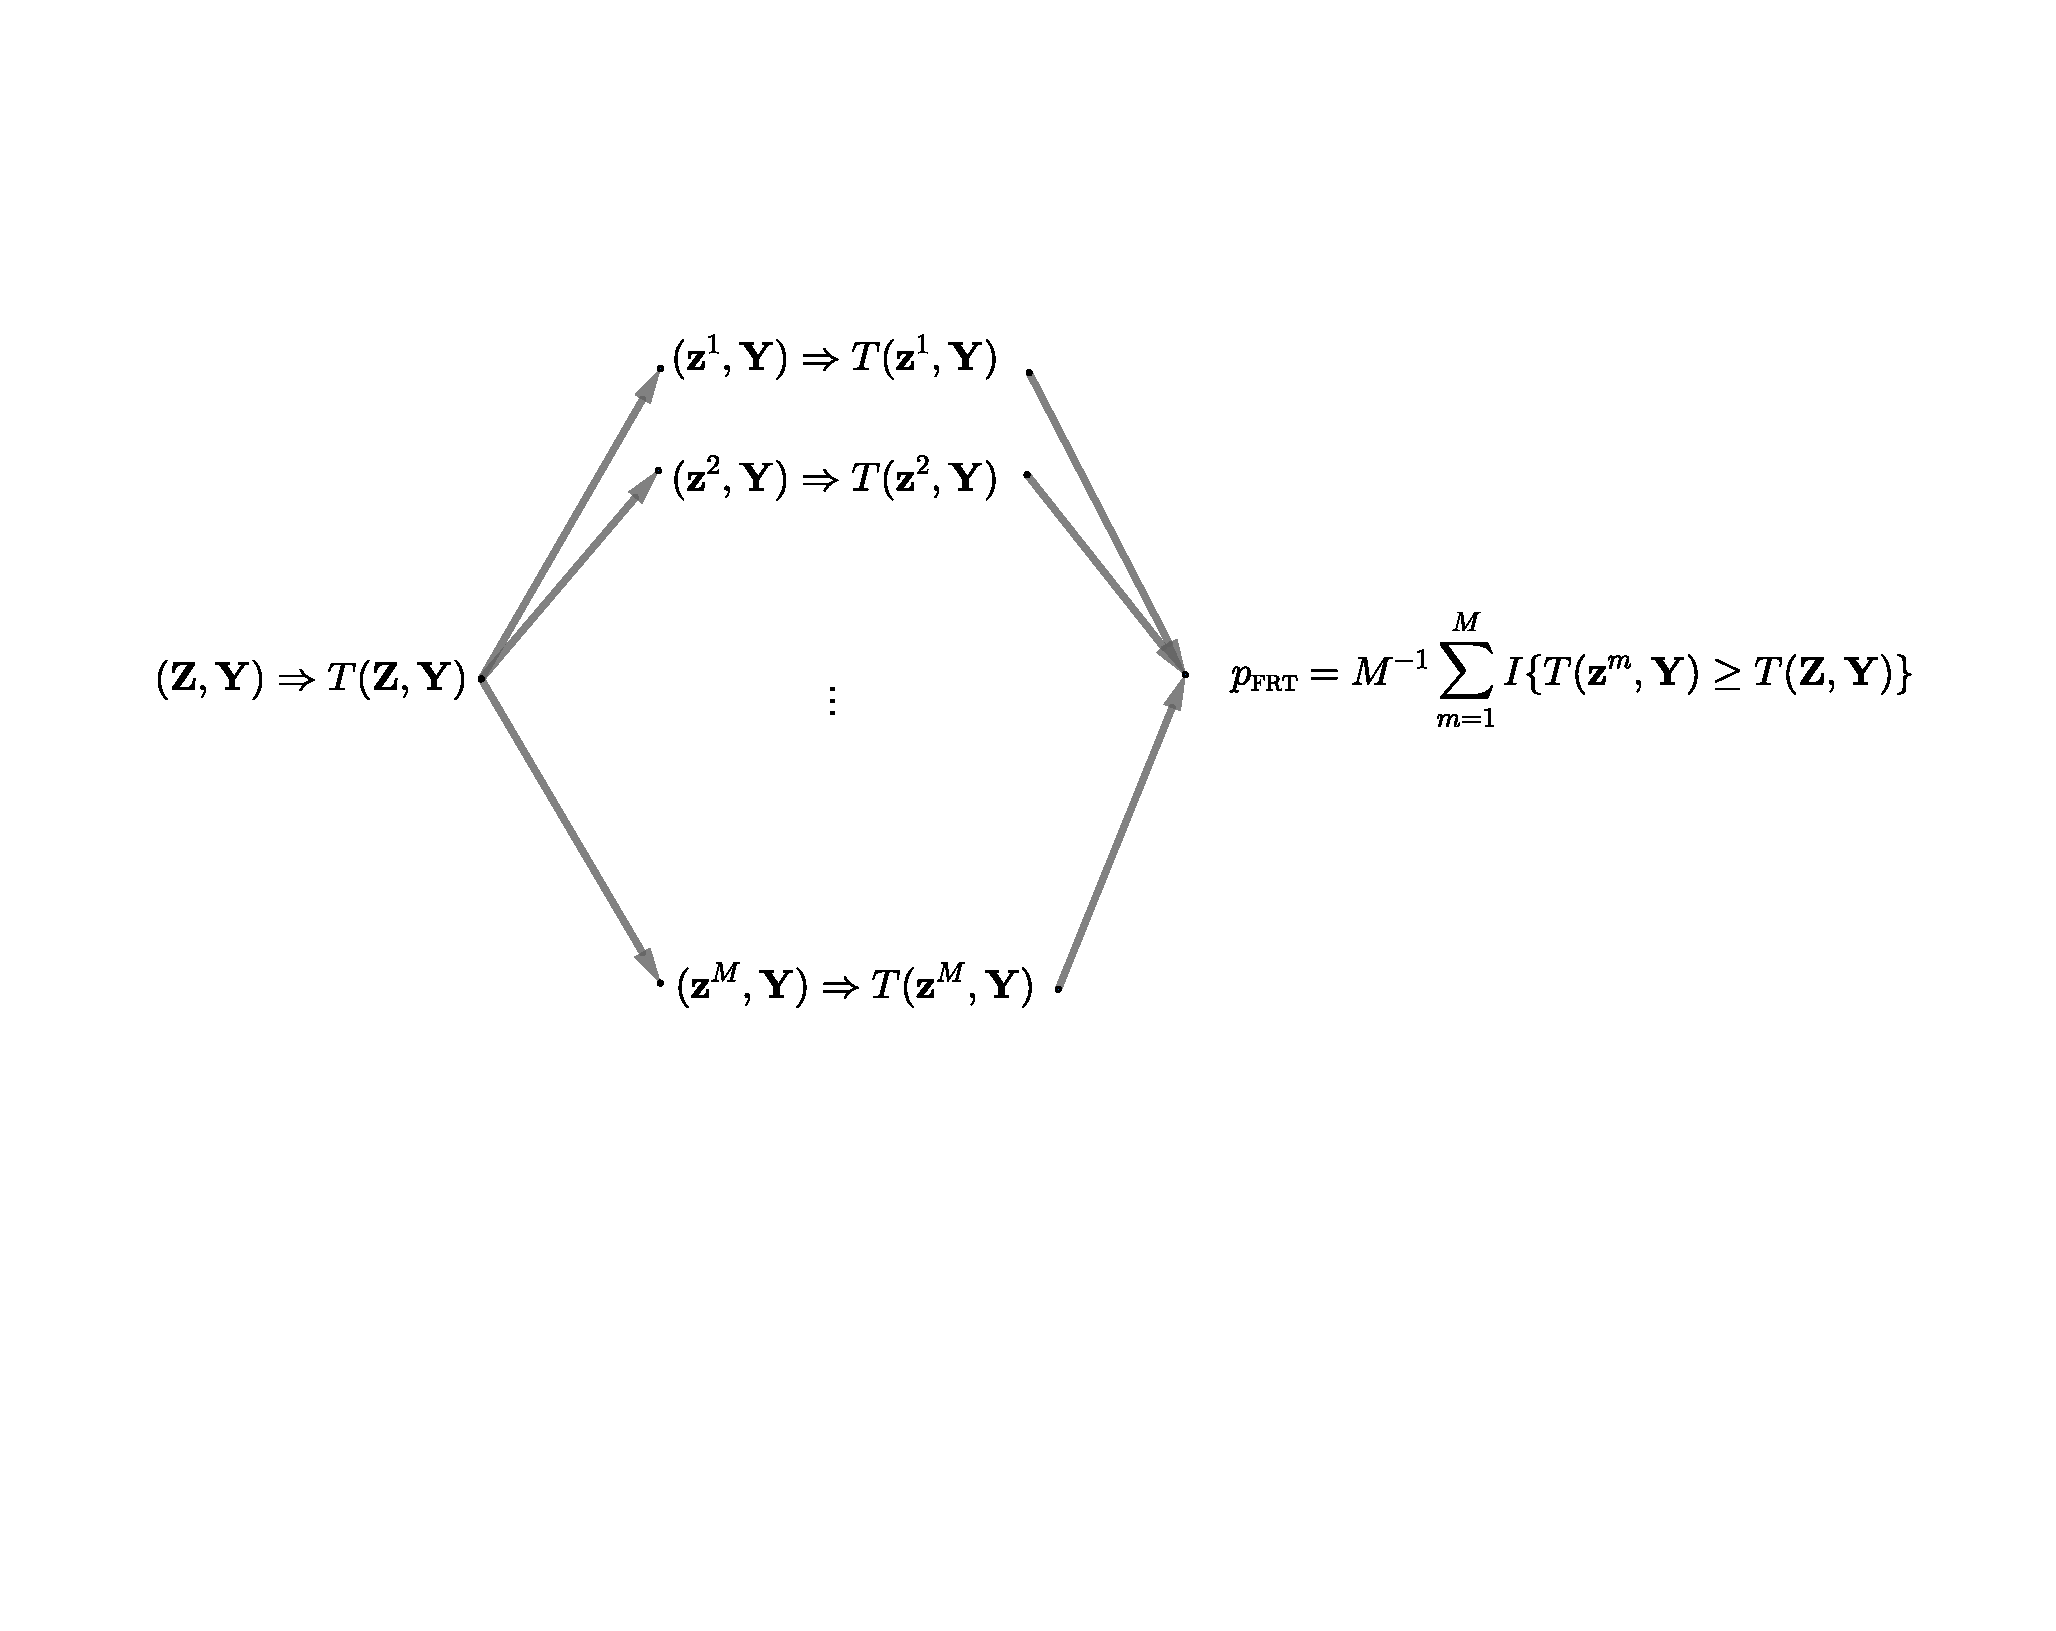
\includegraphics[width =  \textwidth]{figures/frt_fig.pdf}
\caption{ FRT示意图}\label{fig::frt}
\end{figure}




$p$值，即$p_\frt$，在\eqref{eq::exactpvalue}中对任意检验统计量的选择以及任意结果生成过程均适用。该结论还能自然地推广至任意实验情形，这也是后续章节中将反复探讨的主题。重要的是，从\footnote{的意义上来说，该值具有有限样本下的精确性。这正是数理统计学中对$p$值的标准定义。出现不等式的原因通常在于检验统计量的离散性；而当等式成立时，在零假设下$p$值服从$(0,1)$上的均匀分布。设$F(\cdot)$为$T(\bm{Z},\bm{Y})$的分布函数。尽管该分布函数属于阶梯函数，我们仍假定其连续且严格单调递增，就如同它是定义在整个实数轴上的某个连续随机变量的分布函数一般。因此$p_\frt = 1- F(T)$，并且
$$
\pr(p_\frt \leq u) = \pr\{ 1-F(T) \leq u\} = \pr\{  T \geq F^{-1}(1-u)  \} = 1- F( F^{-1}(1-u)) = u.
$$
$T$的离散性确实会在证明过程中引发一些技术性问题，从而导致出现不等式而非等式。具体的技术细节则留作习题\ref{hw::exact-frt}加以探讨。}即在$\HF$条件下，
\begin{eqnarray}\label{eq::p-value-valid}
\pr(p_\frt \leq u) \leq u \quad  \text{ for all } \quad 0 \leq u \leq 1.
\end{eqnarray}




在实践中，$M$的值通常过大（例如，当$n=100, n_1=50$时，我们有$M > 10^{29}$），因此要枚举出处理向量所有可能的取值在计算上是不可行的。我们通常借助蒙特卡洛方法来近似计算$p_\frt$（关于蒙特卡洛方法的基本介绍可参见\ref{sec::monte-carlo-method}节）。具体而言，我们从处理向量的所有可能取值中独立抽取随机样本；或者等价地说，我们对$\bm{Z}$进行随机排列，随后利用下式来近似$p_\frt$：
\begin{equation}\label{eq::mcpvalue}
\hat p_\frt  =  R^{-1} \sum_{r=1}^R   I\{ T(\bm{z}^r,\bm{Y})   \geq T(\bm{Z},\bm{Y})   \},
\end{equation}
其中$\bm{z}^r$代表$R$次对$\bm{Z}$的随机排列。

在\eqref{eq::mcpvalue}中，随着$R$值的增大，$p$值对应的蒙特卡洛误差会迅速减小；详见\ref{para::monte-carlo-error-pfrt}题。由于计算\eqref{eq::mcpvalue}中的$p$值需要用到$\bm{Z}$的排列运算，因此在CRE背景下，FRT有时也被称作{\it 排列检验}。不过，FRT的理念其实比那些用于较复杂实验的排列检验更为通用。 



\section{检验统计量的典型选择}
\label{sec::frt-choiceofstatistic}

根据上述讨论可知，无论选择何种检验统计量，FRT都能产生有限样本下的精确$p$值。这正是FRT的一个特性。不过，这一特性并不应成为随意选择检验统计量的依据。直观而言，我们应当选择那些能够反映$\HF$是否可能被违反的检验统计量。下文我将介绍一些典型的检验统计量选择方式。 


\begin{example}[均值差法]\label{eq::frt-difference-in-means}
均值差统计量即为
$$
\hat{\tau}   = \hat{\bar{Y}}(1) - \hat{\bar{Y}}(0)
$$
其中
$$
 \hat{\bar{Y}}(1)  =  n_1^{-1} \sum_{Z_i=1} Y_i  = n_1^{-1} \sumn Z_iY_i 
$$
表示接受处理时观测结果的样本均值，而
$$
\hat{\bar{Y}}(0) = n_0^{-1}  \sum_{Z_i=0} Y_i   = n_0^{-1}  \sumn (1-Z_i) Y_i 
$$
表示对照组中观测结果的样本均值。
%
%\begin{eqnarray*}
%\hat{\tau}  &=& n_1^{-1} \sum_{Z_i=1} Y_i - n_0^{-1}  \sum_{Z_i=0} Y_i  \\
%&=&  n_1^{-1} \sumn Z_iY_i - n_0^{-1}  \sumn (1-Z_i) Y_i  \\
%&\equiv & \hat{\bar{Y}}(1) - \hat{\bar{Y}}(0).
%\end{eqnarray*}
在$\HF$条件下，其均值为
$$
E(  \hat{\tau}    ) = n_1^{-1}\sumn E(Z_i)Y_i  - n_0^{-1}  \sumn E(1-Z_i) Y_i  = 0
$$
方差则为
\begin{eqnarray*}
\var( \hat{\tau}   ) &=& \var\left\{  n_1^{-1} \sumn Z_iY_i - n_0^{-1}  \sumn (1-Z_i) Y_i  \right\} \\
&=&\var\left(  \frac{n}{n_0}    \frac{1}{n_1} \sumn  Z_i Y_i         \right) \\
&=_*& \frac{n^2}{n_0^2} \left( 1 - \frac{n_1}{n} \right) \frac{s^2}{n_1} \\ 
&=& \frac{n}{n_1 n_0} s^2,
\end{eqnarray*}
其中$=_*$这一结论是根据针对简单随机抽样的\ref{lemma::samplemean}号引理以及$$
\bar{Y} = n^{-1}  \sumn Y_i,\quad 
s^2 = (n-1)^{-1} \sumn (Y_i - \bar{Y})^2 .  
$$得出的。
此外，根据\ref{lemma::finite-population-clt}号引理中所述的有限总体中心极限定理，$\hat{\tau}$的随机化分布近似呈正态分布：
\begin{equation}\label{eq::frt-tau-hat}
\frac{  \hat{\tau}      }{  \sqrt{\frac{n}{n_1 n_0} s^2}    }  
%= \frac{  n_1^{-1} \sum_{Z_i=1} Y_i - n_0^{-1}  \sum_{Z_i=0} Y_i  }{ \sqrt{   \frac{n}{n_1 n_0(n-1)}    \sumn (Y_i - \bar{Y})^2   }  }   
\rightarrow  \N01 
\end{equation}
其分布符合该规律。由于$s^2$在$\HF$条件下为固定值，因此在FRT中将其替换为$$
\frac{  \hat{\tau}      }{  \sqrt{\frac{n}{n_1 n_0} s^2}    }  
$$作为检验统计量同样可行；正如\eqref{eq::frt-tau-hat}所示，该统计量渐进地服从$\textsc{N}(0,1)$分布。如此我们便可计算出近似的$p$值。 
\end{example}


观测到的数据为 $\{  Y_i: Z_i = 1 \}$ 与 $\{ Y_i : Z_i = 0 \}$，因此该问题本质上属于双样本问题。  
在假定结果变量服从独立同分布的正态分布这一前提下（参见第 \ref{sec::bf-problem} 节），经典的、假设方差相等的双样本 $t$ 检验是基于如下公式：
\begin{equation}\label{eq::two-sample-t-equalv}
\frac{  \hat{\tau}      }{  \sqrt{\frac{n}{n_1 n_0(n-2)}  \left[  \sum_{Z_i=1}  \{Y_i - \hat{\bar{Y}}(1)\}^2
+ \sum_{Z_i=0}  \{Y_i - \hat{\bar{Y}}(0)\}^2
    \right]  }    }   \sim t_{n-2}.
\end{equation}
通过一些代数运算（参见习题 \ref{hw::frt-algebraic-detail}），可得到如下展开式：
\begin{equation}\label{eq::frt-algebra-difference-in-means}
(n-1)s^2 = \sum_{Z_i=1}  \{Y_i - \hat{\bar{Y}}(1)\}^2 + \sum_{Z_i=0}  \{Y_i - \hat{\bar{Y}}(0)\}^2
+ \frac{n_1 n_0}{n} \hat{\tau}^2 .
\end{equation}
当样本量 $n$ 较大时，我们可以忽略 $\N01$ 与 $t_{n-2}$ 之间的差异，以及 $n-1$ 与 $n-2$ 之间的差异。  
此外，在 $\HF,$ 条件下，$\hat{\tau}$ 依概率收敛至零，因此从渐近角度而言 $ n_1 n_0 / n \hat{\tau}^2$ 可忽略不计。于是，在 $\HF,$ 条件下，例 \ref{eq::frt-difference-in-means} 中计算出的近似 $p$ 值会接近于经典等方差双样本 $t$ 检验所算出的 $p$ 值；后者可通过 \ri{t.test} 结合 \ri{var.equal = TRUE} 来计算得出。而在 $\tau$ 不为零的备择假设下，展开式 \eqref{eq::frt-algebra-difference-in-means} 中的附加项 $\frac{n_1 n_0}{n} \hat{\tau}^2$ 可能导致 FRT 的功效低于常规的 $t$ 检验；\citet{Ding:2014} 曾指出这一点。 


基于上述讨论，采用$\hat{\tau}$的FRT实际上是利用了合并方差，而忽略了两组之间的异方差性。在经典统计学中，具有异方差性正态分布结果的双样本问题被称为贝伦斯-费舍尔问题（详见\ref{sec::bf-problem}节）。在该问题中，最常用的检验统计量即为下述的学生化统计量。 



\begin{example}[学生化统计量]
\label{eg::studentized-statistic}
该学生化统计量\footnote{此处使用$t$这一符号是有意为之，因为它与$t$分布相关。不过不应将其与符号$t_\nu$相混淆，后者表示自由度为$\nu$的$t$分布。}的计算公式为
$$
t = \frac{    \hat{\bar{Y}}(1)  -   \hat{\bar{Y}}(0)    }{  \sqrt{  \frac{  \hat{S}^2(1)  }{n_1}  + \frac{\hat{S}^2(0)}{n_0}  }   },
$$
其中
$$
\hat{S}^2(1) = (n_1 - 1)^{-1} \sum_{Z_i =1} \{ Y_i  -\hat{\bar{Y}}(1)   \}^2,\quad
\hat{S}^2(0) = (n_0 - 1)^{-1} \sum_{Z_i =0} \{ Y_i  -\hat{\bar{Y}}(0)   \}^2 
$$
分别代表处理组与对照组中观测结果的样本方差。在$\HF$条件下，有限总体中心极限定理再次表明：$t$呈渐近正态分布：
$$
t \rightarrow \N01 
$$
即服从该分布。
随后我们便可计算出一个近似的$p$值，该值接近于由\ri{t.test}及\ri{var.equal = FALSE}所得出的$p$值。
\end{example}



一个极其重要的观点是：即便基础分布并非正态分布，FRT方法也能为那些使用\ri{t.test}并结合\ri{var.equal = TRUE}或\ri{var.equal = FALSE}的传统$t$检验提供合理性依据。通常的统计学教材均基于正态分布这一假设来阐述$t$检验的合理性，但该假设在现实应用中可能过于严苛。幸运的是，只要有限总体中心极限定理成立，我们依然可以运用$t$检验程序。即便我们不认同这些中心极限定理，仍可借助$\hat{\tau}$与$t$作为FRT中的检验统计量，从而获得有限样本下的精确$p$值。 


我们将在第\ref{chapter::unification-fisher-neyman}章从另一个角度来阐述这一学生化统计量的合理性。该章节的理论表明，在FRT中使用$t$能够增强对两组间异方差性的稳健性。 


下述检验统计量对于由重尾分布的结果数据所产生的异常值具有稳健性。 




\begin{example}[威尔科克森秩和]\label{example::wilcoxon-cre}
均值差统计量$ \hat{\tau} $利用原始结果的样本均值进行计算，其抽样分布取决于结果的方差。而学生化统计量$t$则利用原始结果的样本均值与方差进行计算，其抽样分布取决于结果的更高阶矩。正因如此，$ \hat{\tau} $与$t$对异常值较为敏感。 

另一种常用的检验统计量是基于合并后观测结果的秩次。令$R_i$表示$Y_i$在合并样本$\bm{Y}$中的秩次：
$$
R_i = \#\{j : Y_j \leq Y_i  \}.
$$
威尔科克森秩和统计量即为处理组中各观测值秩次的总和：
$$
W = \sumn Z_i R_i.
$$
为简化代数运算，我们假设观测结果中不存在结值。\footnote{
无论是否存在结值，FRT均可应用。若存在结值，我们既可以向原始结果添加微小的随机噪声，也可以采用结值对应的平均秩次。
关于存在结值的情况，可参见\citet[][Chapter 1 Section 4]{lehmann2006nonparametrics}。
}
由于合并样本中所有秩次的总和恒定为$1+2+\cdots + n = n(n+1)/2$，因此威尔科克森统计量实际上等同于处理组与对照组中秩次均值的差值。
在$\HF$条件下，各$R_i$均为固定值，因此
%We can use Lemma \ref{lemma::samplemean} to calculate the moments of $W$ under $\HF$: because the $R_i$'s are fixed, 
$W$的均值为
$$
E(W)  =  \sumn E(Z_i) R_i  =\frac{n_1}{n}  \sumn  i   = \frac{n_1}{n} \times \frac{n(n+1)}{2} = \frac{n_1(n+1)}{2} 
$$
其方差为
\begin{eqnarray*}
\var(W) &=& \var\left( n_1 \frac{1}{n_1} \sumn Z_i R_i  \right) \\
&=_*&  n_1^2  \left( 1-\frac{n_1}{n} \right)  \frac{1}{n_1}  \frac{1}{n-1} \sumn \left(R_i - \frac{n+1}{2}  \right)^2\\
&=&  \frac{n_1 n_0}{n(n-1)} \sumn \left(i - \frac{n+1}{2}  \right)^2\\
&=&   \frac{n_1 n_0}{n(n-1)}   \left\{ \sumn i^2 - n \left(  \frac{n+1}{2}\right)^2     \right\}\\
&=&  \frac{n_1 n_0}{n(n-1)}  \left\{     \frac{n(n+1)(2n+1)}{6} -    n \left( \frac{n+1}{2}   \right)^2 \right\}  \\
&=& \frac{n_1 n_0 (n+1)}{12},
\end{eqnarray*}
其中$=_*$这一结论可由引理\ref{lemma::samplemean}推导得出。
此外，在$\HF$的条件下，有限总体中心极限定理保证了$\widehat{\tau}$的随机化分布近似服从正态分布：
\begin{eqnarray}
\label{eq::wilcox-normal}
\frac{  \sumn Z_i R_i - \frac{n_1(n+1)}{2}   }{  \sqrt{  \frac{n_1 n_0 (n+1)}{12}   }}   \rightarrow \N01 
\end{eqnarray}
即服从该分布。
基于\eqref{eq::wilcox-normal}，我们可以进行渐近检验。在\ri{R}中，函数\ri{wilcox.test}能够依据统计量$W - n_1(n_1+1)/2$来计算精确的以及渐近的$p$值。通过一些渐近分析，\citet{lehmann2006nonparametrics}证实：在多种数据生成过程下，使用$W$的FRT均具备较为理想的检验效能。
\end{example}





\begin{example}
 [Kolmogorov--Smirnov 统计量]
\label{eg::ks-CRE}
处理可能以不同方式影响结果，因此用经验分布概括处理组与对照组的结果是很自然的：
$$
\hat{F}_1( y) = n_1^{-1} \sumn Z_i I(Y_i \leq y),\quad
\hat{F}_0( y ) = n_0^{-1} \sumn (1-Z_i) I(Y_i \leq y) . 
$$
比较这两个经验分布，就得到著名的 Kolmogorov--Smirnov 统计量
$$
D = \max_y  \Big |
\hat{F}_1( y) 
- \hat{F}_0( y ) 
\Big |.
$$
推导$D$的分布是一个颇具挑战的数学问题。当$n_1\rightarrow \infty$、$n_0\rightarrow \infty$时，其分布函数收敛于
$$
\pr\left(  \sqrt{\frac{n_1 n_0}{n}}  D \leq  x   \right  ) \rightarrow   \frac{\sqrt{2\pi}}{x}   \sum_{j=1}^\infty  e^{     - (2j-1)^2 \pi^2 / (8x^2) }     ,
$$
据此可计算渐近$p$值\citep{van2000asymptotic}。在\ri{R}中，\ri{ks.test}函数可以计算精确和渐近$p$值。
\end{example}







\section{拉隆德实验数据的案例分析}
\label{sec::frt-lalonde-experiment}

下面用\citet{lalonde1986evaluating}的实验数据说明 FRT。数据可在\ri{Matching}包\citep{sekhon2011multivariate}中获得： 

\begin{lstlisting}
> library(Matching)
> data(lalonde)
> z = lalonde$treat
> y = lalonde$re78
\end{lstlisting}

此处\ri{z}为指示实验单位是否接受培训处理的二值向量；\ri{y}为实验单位1978年的实际收入值。图\ref{fig::lalonde-histograms}展示了处理与对照组的收入分布直方图。 


\begin{figure}[ht]
\centering 
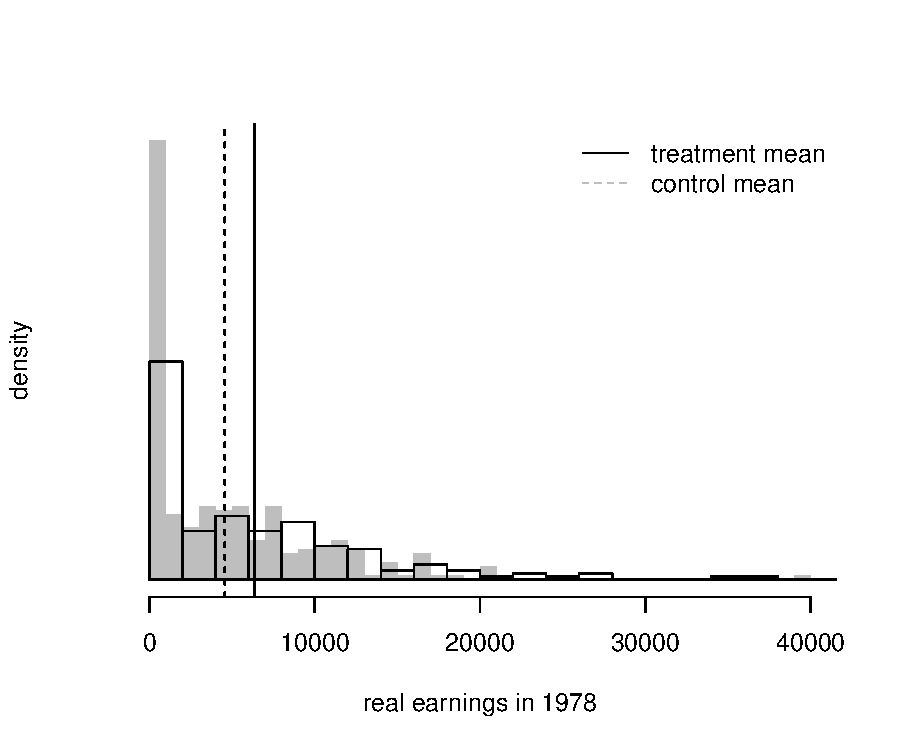
\includegraphics[width =  \textwidth]{figures/lalonde_histograms.pdf}
\caption{拉隆德实验数据中处理组（白色）与对照组（灰色）的收入分布直方图；垂直线分别为两组样本均值：实线为处理组，虚线为对照组。}\label{fig::lalonde-histograms}
\end{figure}



下述代码计算了四种典型统计量的观测值：
\begin{lstlisting}
> tauhat = t.test(y[z == 1], y[z == 0], 
+                 var.equal = TRUE)$statistic
> tauhat
       t 
2.835321 
> student = t.test(y[z == 1], y[z == 0],
+                 var.equal = FALSE)$statistic
> student
       t 
2.674146 
> W = wilcox.test(y[z == 1], y[z == 0])$statistic
> W
      W 
27402.5 
> D = ks.test(y[z == 1], y[z == 0])$statistic
> D
        D 
0.1321206 
\end{lstlisting}

随机置换处理向量，即可得到检验统计量随机化分布的蒙特卡洛近似，结果分别存放在\ri{Tauhat}、\ri{Student}、\ri{Wilcox}和\ri{Ks}四个向量中。 
\begin{lstlisting}
> MC = 10^4
> Tauhat   = rep(0, MC)
> Student  = rep(0, MC)
> Wilcox   = rep(0, MC)
> Ks       = rep(0, MC)
> for(mc in 1:MC)
+ {
+   zperm       = sample(z)
+   Tauhat[mc]  = t.test(y[zperm == 1], y[zperm == 0], 
+                        var.equal = TRUE)$statistic 
+   Student[mc] = t.test(y[zperm == 1], y[zperm == 0], 
+                        var.equal = FALSE)$statistic
+   Wilcox[mc]  = wilcox.test(y[zperm == 1], 
+                             y[zperm == 0])$statistic 
+   Ks[mc]      = ks.test(y[zperm == 1], 
+                         y[zperm == 0])$statistic
+ }
\end{lstlisting}



基于 FRT 的单侧$p$值均小于 0.05： 
\begin{lstlisting}
> exact.pv = c(mean(Tauhat >= tauhat),
+              mean(Student >= student),
+              mean(Wilcox >= W),
+              mean(Ks >= D))
> round(exact.pv, 3)
[1] 0.002 0.002 0.006 0.040
\end{lstlisting}
也可以不使用蒙特卡洛方法，直接计算渐近$p$值，它们同样均小于 0.05： 
\begin{lstlisting}
> asym.pv = c(t.test(y[z == 1], y[z == 0], 
+                    var.equal = TRUE)$p.value, 
+             t.test(y[z == 1], y[z == 0], 
+                    var.equal = FALSE)$p.value,
+             wilcox.test(y[z == 1], y[z == 0])$p.value,
+             ks.test(y[z == 1], y[z == 0])$p.value)
> round(asym.pv, 3)
[1] 0.005 0.008 0.011 0.046
\end{lstlisting}

这些$p$值的差异既来自渐近近似，也来自\ri{t.test}和\ri{wilcox.test}默认进行双侧检验。为作公平比较，需要将前三个$p_\frt$乘以$2$。 


图\ref{fig::randomizationdistribution-lalonde}给出了四个检验统计量随机化分布的直方图及其观测值。虽然原始结果数据的分布远非正态分布（见图\ref{fig::lalonde-histograms}），前三个统计量的正态近似仍很好。一般而言，图\ref{fig::randomizationdistribution-lalonde}这样的图形能更清楚地展示检验尖锐零假设所需的信息。近期\citet{bind2020possible}甚至在论文标题中倡议：“只要可能，就报告 Fisher 精确$p$值，并展示其对应的零假设随机化分布。”我赞同这一建议。 

\begin{figure}[ht]
\centering 
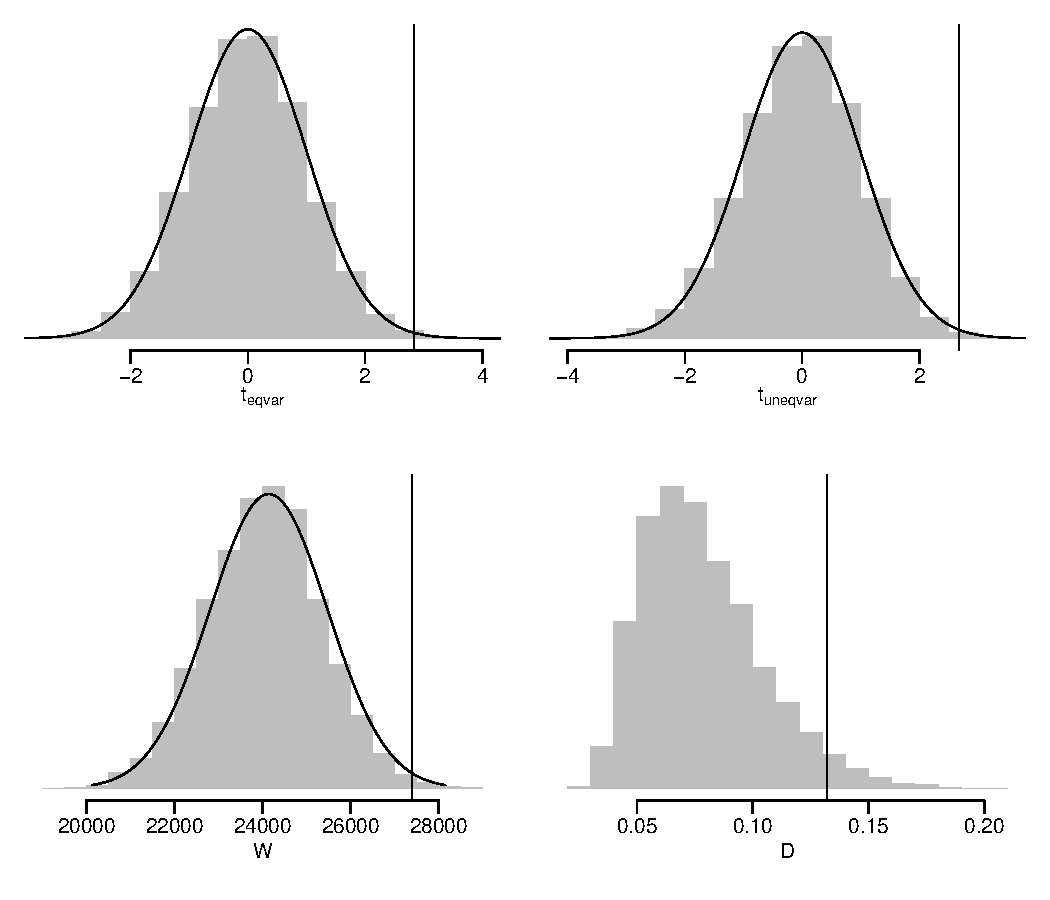
\includegraphics[width =  \textwidth]{figures/FRT_lalonde.pdf}
\caption{基于 LaLonde 实验数据的四个检验统计量的随机化分布} \label{fig::randomizationdistribution-lalonde}
\end{figure}





\section{随机实验与 FRT 的简史}


\subsection{James Lind 的实验}\label{section::lind}


James Lind（1716—1794）是一位苏格兰医生，也是英国皇家海军海上卫生研究的先驱。在他所处的时代，坏血病是水手死亡的主要原因之一。他开展了一项较早且细节记录清楚的随机实验，在维生素 C 被发现之前，就得出柑橘类水果能够治疗坏血病的结论。 


在\citet{lind1753treatise}中，他描述了将$12$名坏血病患者分到$6$组的随机实验。略去部分细节，$6$组分别为：
\begin{enumerate}
[(1)]
\item
两人每天饮用一夸脱苹果酒； 

\item
两人每天服用三次硫酸，每次二十五滴；

\item
两人每天服用三次醋，每次两匙；

\item
两人每天饮用半品脱海水；


\item
两人每天食用两个橙子和一个柠檬；

\item 
两人每天食用一种辛辣糊剂，并饮用大麦水。
\end{enumerate}

六天后，第五组患者康复，而其他组没有康复。若将处理简化为
$$
Z_i  = 1(\text{unit } i \text{ received citrus fruits})
$$
并将结果简化为
$$
Y_i = 1(\text{unit } i \text{ recovered after six days}),
$$
就得到如下二乘二列联表：

\begin{center}
\begin{tabular}{lcc}
\hline 
      & $Y =1$ & $Y =0$\\\hline
$Z =1$ & $2$ & $0$\\ 
$Z =0$ & $0$ & $10$\\
\hline 
\end{tabular}
\end{center}


这是该实验中能够观测到的最极端的二乘二列联表，数据为柑橘类水果治疗坏血病的正向效应提供了强有力的证据。从统计学角度，应如何衡量证据的强度？


按照 FRT 的逻辑，若处理完全没有效应（即$\HF$成立），如此极端的二乘二表出现的概率为
$$
 \frac{1}{\binom{12}{2}} = \frac{1}{66} = 0.015
$$
这就是$p_\frt$。在$\HF$下，这样的结果相当出乎意料：在$0.05.$水平上，我们很容易拒绝$\HF$。



\subsection{女士品茶}\label{section::lady-tasting-tea}


\citet{Fisher:1935}描述了著名的{\it 女士品茶}实验。\footnote{后来\citet{salsburg2001lady}撰写现代统计学史时，将这一名称用作书名。}一位女士声称，她能分辨两种制作奶茶的方法：先加奶和先加茶。多数人可能会觉得这个说法有些奇怪。作为统计学家，Fisher 设计了一项实验，检验这位女士是否真的能区分两种做法。 

他准备了$8$杯茶，其中$4$杯先加奶，另$4$杯先加茶，再将$8$杯茶按随机顺序呈给女士，请她选出先加奶的$4$杯。最终实验结果可汇总为下列二乘二表： 

\begin{tabular}{lccc}
\hline 
      &    先加奶（女士判断）&    先加茶（女士判断） & 列合计 \\ \hline
      先加奶（Fisher 安排） & $X$ & $4-X$ & 4\\ 
   先加茶（Fisher 安排） & $4-X$ & $X$ & 4\\
   行合计 & 4 & 4 &8 \\
   \hline 
\end{tabular}

$X$的可能取值为$0, 1, 2, 3, 4$。实际实验得到$X = 4$，这是最极端的数据，强烈表明女士确实能够区分两种奶茶做法。我们再次面临同一个问题：如何衡量证据的强度？


在女士无法区分两种做法的零假设下，$\binom{8}{4} = 70$种可能排列中，只有一种会得到$X=4$的二乘二表。因此，$p$值为
$$
p_\frt = \frac{1}{70} = 0.014.
$$
在$0.05$的显著性水平上，我们拒绝零假设。 



\subsection{Fisher 实验设计的两个原则}\label{sec::fisherian-principles-experiments}


在第\ref{section::lind}和\ref{section::lady-tasting-tea}节的两个例子中，$p_\frt$的有效性都由实验的随机化保证。这突出了 Fisher 实验设计的第一个原则：{\it 随机化}。




 
 
 


此外，从某种意义上说，上述两项实验已经是能够给出有统计意义结果的最小实验。例如，若 Lind 只给六个组各分配一名患者，则最小$p$值为
$$
\frac{1}{\binom{6}{1}}  =\frac{1}{6} = 0.167;
$$
若 Fisher 只准备$6$杯茶，其中$3$杯先加奶、另$3$杯先加茶，则最小$p$值为
$$
\frac{1}{\binom{6}{3}} = \frac{1}{20} = 0.05.
$$
此时无法在$0.05$水平上拒绝零假设。这突出了 Fisher 实验设计的第二个原则：{\it 重复}。也就是说，为使 FRT 具有检验功效，实验中必须有足够多的单位。 

 

第\ref{chapter::stratification-poststratification}章将讨论 Fisher 实验设计的第三个原则：{\it 区组化}。


 

 

\section{讨论}

\subsection{其他尖锐零假设与置信区间}\label{sec::frt-invert-interval}


上文着重讨论尖锐零假设$\HF$。实际上，FRT 的逻辑也适用于其他尖锐零假设。例如，对于已知向量$\bm{\tau} = (\tau_1, \ldots, \tau_n)$，可检验
$$
H_0(\bm{\tau}): Y_i(1) - Y_i(0) = \tau_i \text{ for all } i=1,\ldots, n
$$
在$H_0(\bm{\tau})$下，每个单位的因果效应都已知，因此可以根据观测数据填补所有缺失的潜在结果。潜在结果确定后，任意检验统计量$T = T(\bm{Z}, \bm{Y}(1), \bm{Y}(0))$的分布都完全由处理分配机制决定，从而可计算对应的$p_\frt$。它是$\bm{\tau} $的函数，记为$p_\frt(\bm{\tau} )$。若能列出所有可能的$\bm{\tau}$，就可得到一系列$p_\frt(\bm{\tau} )$。根据假设检验与置信集合的对偶性（见第\ref{section::duality-ci-testing}节），可构造平均因果效应的$(1-\alpha)$水平置信集合：
$$
\left \{ \tau = n^{-1}\sum_{i=1}^n \tau_i :  p_\frt(\bm{\tau} ) \geq \alpha \right \} .
$$
这个策略在概念上很直接，但所有可能的$\bm{\tau}$数量庞大，实践中存在计算困难。对于二元结果，\citet{Rigdon:2015}和\citet{li2016exact}提出了基于 FRT 构造$\tau$置信区间的可计算方法。对于一般无界结果，这一策略往往在计算上不可行。 


一种常用的简化\citep{rosenbaum2002design, Rosenbaum:2010}是只考虑个体因果效应恒定的一类尖锐零假设：
$$
H_0(c): Y_i(1) - Y_i(0) =  c\text{ for all } i=1,\ldots, n
$$
其中$c$是已知常数。给定$c$，可以计算$p_\frt(c)$。利用对偶性，可得到平均因果效应的$(1-\alpha)$水平置信集合：
$$
\{ c :  p_\frt(c ) \geq \alpha \} .
$$
这一过程只涉及一维搜索，因此在计算上可行。然而，个体因果效应恒定的假设过强。特别是，对于二元结果，只有所有单位的效应都为$0,$、都为$-1$或都为$1$时，该假设才能成立。一般而言，恒定个体因果效应假设对数据施加了可检验的限制，因此可能被观测数据拒绝；\citet{ding2015randomization}提出了正式的统计检验。 



\subsection{其他检验统计量}\label{section::other-statistic}


FRT 是一种一般性的策略，适用于任何随机实验和任何检验统计量。第\ref{sec::frt-choiceofstatistic}节已经介绍了若干统计量，其实统计量的定义还可以更一般。例如，令处理前协变量矩阵为$\bm{X}$，第$i$行为单位$i$的协变量$X_i$，$(i = 1, \ldots, n)$。\footnote{在因果推断中，只有不受处理影响的变量$X_i$才称为协变量。也就是说，若它有两个潜在结果$X_i(1)$和$X_i(0)$，则二者必须满足$X_i(1) = X_i(0)$。标准统计教材往往不区分处理与协变量，因为二者通常都出现在结果回归模型的右侧，并都被称为协变量。本书加以区分，因为它们在因果推断中发挥不同作用。}此时可以令检验统计量$T(\bm{Z}, \bm{Y}, \bm{X})$为处理向量、结果向量和协变量矩阵的函数，习题\ref{hw::frt-covariates}给出了一个例子。 



\subsection{最后的说明}对于一般的实验，$\bm{Z}$未必在所有由$n_1$个 1 和$n_0$个 0 构成的排列上均匀分布，但实验者完全知道其分布。因此，总能模拟该分布，进而得到尖锐零假设下任意检验统计量的分布。有限样本精确$p$值为
$$
p_\textsc{frt} = \pr'\{  T(\bm{Z}', \bm{Y}) \geq T(\bm{Z}, \bm{Y}) \}
$$
其中$\pr'$表示在给定数据后，对$\bm{Z}'$的分布求平均。后续章节将讨论其他实验。这里强调，FRT 的适用范围不限于本书介绍的几种具体实验。 

 
FRT 可以使用任意检验统计量，但这并未回答实际分析中应如何选择统计量。如果目的是发现与尖锐零假设不相容的结果，就应选择在备择假设下功效较高的统计量。一般没有一种统计量的功效能始终优于其他统计量，因为功效取决于备择假设。第\ref{sec::frt-choiceofstatistic}节的四个统计量针对不同备择假设：例如，$\hat{\tau}$和$t$针对平均处理效应不为零的备择；$W$则针对结果呈重尾分布、因果效应恒定的备择。指定一个工作备择假设通常有助于构造检验统计量，但 FRT 的有效性并不要求该备择假设准确。习题\ref{hw::frt-covariates}和\ref{hw::frt-glm}说明了如何利用工作备择假设或统计模型构造统计量。 
 



\section{作业习题}



\paragraph{$p_\frt$的精确性}
\label{hw::exact-frt}

证明 \eqref{eq::p-value-valid}。 



\paragraph{$\hat p_\frt$的蒙特卡洛误差}\label{para::monte-carlo-error-pfrt}

给定数据后，$p_\frt$是固定数，而它在\eqref{eq::mcpvalue}中的蒙特卡洛估计$\hat p_\frt$仍是随机的。证明
$$
E_{\text{mc}} (\hat p_\frt) =   p_\frt
$$
以及
$$
\var_{\text{mc}} (\hat p_\frt)  \leq \frac{1}{4R},
$$
下标“mc”表示蒙特卡洛方法引入的随机性：$\hat p_\frt$之所以随机，是因为各$\bm{z}^r$是从$\bm{Z}$的所有可能取值中独立随机抽取的$R$个向量。


注：$p_\frt$的随机性来自$\bm{Z}$，但本题以数据为条件，故$p_\frt$成为固定数。$\hat p_\frt$的随机性则来自各$\bm{z}^r$是$\bm{Z}$的随机置换。习题\ref{para::monte-carlo-error-pfrt}证明，对蒙特卡洛随机性求平均时，$\hat p_\frt$是$p_\frt$的无偏估计量，并给出了$\hat p_\frt$方差的上界。\citet[][Theorem 2]{luo2021leveraging}给出了更精细的蒙特卡洛误差界。




\paragraph{$p_\frt$的有限样本有效蒙特卡洛近似}\label{para::finite-sample-exact-monte-carlo-frt}


尽管由习题\ref{para::monte-carlo-error-pfrt}可知$\hat p_\frt$是$p_\frt$的无偏估计量，但当$R$有限时，蒙特卡洛误差可能使它不满足对所有$u\in (0,1)$都有$\pr(\hat p_\frt \leq u) \leq u$的要求，因而未必是有效$p$值。下面的修正蒙特卡洛近似始终是有限样本有效的$p$值。\citet{phipson2010permutation}在置换检验中指出了这一技巧。



定义
$$
\tilde p_\frt  =  \frac{  1 + \sum_{r=1}^R   I\{ T(\bm{z}^r,\bm{Y})   \geq T(\bm{Z},\bm{Y})   \}  }{1+R}
$$
其中各$\bm{z}^r$是$\bm{Z}$的$R$次随机置换。证明：无论$R$取何值，蒙特卡洛近似$\tilde p_\frt $始终是有限样本有效的$p$值，即对所有$u\in (0,1)$均有$\pr(\tilde p_\frt \leq u) \leq u$。


 
注：可利用以下两个基本概率结论证明习题\ref{para::finite-sample-exact-monte-carlo-frt}的结论。 


\begin{lemma}
\label{lemma::binomial-order}
设两个二项随机变量$X_1\sim \text{Binomial}(R, p_1)$和$X_2\sim \text{Binomial}(R, p_2)$满足$p_1\geq p_2$，则对所有$x.$，均有$\pr(X_1\leq x) \leq  \pr(X_2\leq x) $。
\end{lemma}

\begin{lemma}
\label{lemma::uniform}
若$p\sim \text{Uniform}(0,1)$且$X\mid p \sim \text{Binomial}(R, p)$，则从边际分布来看，$X$在$\{ 0,1,\ldots, R  \}$上服从均匀分布。 
\end{lemma}

 


\paragraph{费舍尔精确检验}
\label{hw::frt-fisherexacttest}

考虑结果为二元变量的完全随机实验，将数据汇总为以下二乘二表：
 \begin{center}
\begin{tabular}{lccc}
\hline 
        & $Y =1$ & $Y =0$& 合计\\\hline
$Z =1$ & $n_{11}$ & $n_{10}$ & $n_1$\\ 
$Z =0$ & $n_{01}$ & $n_{00}$ & $n_0$\\ 
\hline 
\end{tabular}
\end{center}
在$\HF$下，证明任意检验统计量$T(n_{11}, n_{10}, n_{01}, n_{00})$都是$n_{11}$与其他非随机常数的函数，且$n_{11}$的精确分布为超几何分布。写出该超几何分布的参数。 

注：\citet{barnard1947significance}和\citet{Ding:2015}指出，在具有二元结果的完全随机实验中，Fisher 精确检验（见第\ref{sec::fisher-exact-test}节）与 FRT 等价。 





\paragraph{女士品茶实验的更多细节}
\label{hw::more-tea}

回顾第\ref{section::lady-tasting-tea}节的例子。计算$k=0,1,2,3,4$时的$\pr(X=k)$。 


\paragraph{协变量调整后的 FRT}
\label{hw::frt-covariates}


本题补充第\ref{section::other-statistic}节的细节。  


第\ref{sec::frt-lalonde-experiment}节使用四种检验统计量，通过 FRT 重新分析了 LaLonde 实验数据。若有额外协变量，至少还可以采用以下两种策略，使 FRT 更一般。假定所有潜在结果和协变量均为固定数。 

第一种策略是使用基于线性回归残差的检验统计量。将结果对协变量作线性回归，得到残差，并把残差视为“伪结果”。然后用残差定义前述四种统计量，分别实施 FRT，报告相应的$p$值。


第二种策略是将结果对处理和协变量作线性回归，以处理的回归系数作为检验统计量实施 FRT，并报告相应$p$值。 


为什么上述两种策略给出的五个$p$值都具有有限样本精确性？请说明理由。 



\paragraph{使用广义线性模型的 FRT}
\label{hw::frt-glm}


使用习题\ref{hw::frt-covariates}的数据集，将结果改为表示\ri{re78}是否为正的二元指标。将结果对处理与协变量作逻辑回归。处理系数是否显著？对应的$p$值是多少？再以处理系数作为检验统计量，计算 FRT 的$p$值。 




\paragraph{一个代数细节}
\label{hw::frt-algebraic-detail}

验证 \eqref{eq::frt-algebra-difference-in-means}。 



\paragraph{推荐阅读}

近期论文\citet{bind2020possible}倡导在分析复杂实验时，同时报告$p$值并展示相应的随机化分布。 

